\documentclass[12pt,a4paper]{article}

\usepackage[margin=1in]{geometry}
\usepackage[T1]{fontenc}
\usepackage[utf8]{inputenc}
\usepackage{lmodern}
\usepackage{setspace}
\usepackage{booktabs}
\usepackage{array}
\usepackage{float}
\usepackage{xcolor}
\usepackage{hyperref}
\usepackage{amsmath}
\usepackage{xurl}
\usepackage{tikz}
\usepackage{pgfplots}
\usepackage{enumitem}

\pgfplotsset{compat=1.18}
\usetikzlibrary{positioning,arrows.meta}
\setstretch{1.15}
\hypersetup{
  colorlinks=true,
  linkcolor=blue!50!black,
  urlcolor=blue!50!black
}

\title{\textbf{Heatwave Heat Map Life: An AI-Driven Heatwave Prediction and Public Warning System for Thailand}}
\author{Chonradsadornumrung School}
\date{March 7, 2026}

\begin{document}

\maketitle

\begin{abstract}
Heatwave Heat Map Life is an AI-supported heatwave prediction and public warning system designed for Thailand. The backend ingests ERA5 NetCDF data, crops them to the Thailand domain, builds spatiotemporal feature windows, and trains an imbalance-aware Balanced Random Forest classifier that estimates the probability of heatwave events. A Flask API exposes summary predictions, multi-day forecasts, and GeoJSON map layers that can be consumed by a dashboard or mobile-facing application. Using the latest operational checkpoint available in the repository, the system achieves a test accuracy of 0.896, a test F1 score of 0.672, and a PR-AUC of 0.779. These results indicate that the project already provides meaningful heat-risk signal extraction, while still leaving room for stronger calibration, richer labels, and broader validation.
\end{abstract}

\noindent\textbf{Keywords:} heatwave prediction, ERA5, balanced random forest, Thailand, climate adaptation

\section{Introduction}
Heatwaves are among the most serious climate hazards for tropical countries because they affect public health, outdoor labor, energy demand, and daily safety. In Thailand, prolonged high temperatures can produce dangerous conditions even before temperatures reach the extremes often discussed in temperate-climate research. Global health guidance increasingly treats extreme heat as a direct public-health threat rather than a secondary inconvenience, especially for vulnerable populations and heat-exposed workers \cite{whoheat}. A useful early-warning system therefore needs more than a raw temperature forecast. It must also translate climate signals into a clear estimate of risk that can support practical protective action.

This project addresses that need by combining climate-data preprocessing, AI-based event detection, and a service layer that returns public-facing warning outputs. The system is designed to transform large weather fields into understandable products such as heatwave probabilities, discrete risk levels, and map-based warnings. That framing makes the project relevant not only as a machine-learning exercise, but also as an environmental communication tool.

\section{Literature Review}
Research on heatwave forecasting commonly relies on physically grounded atmospheric datasets and event-based definitions of extreme heat. Reanalysis products such as ERA5 are especially valuable because they provide long, spatially consistent records of temperature, humidity, precipitation, and related variables across regions where local station coverage may be uneven \cite{hersbach2020}. These datasets are frequently used as inputs for both statistical forecasting and machine-learning pipelines.

A second theme in the literature concerns how to define a heatwave. Many studies move beyond a single daily temperature threshold and instead combine threshold intensity with duration and spatial extent. This is important because heat-related risk accumulates through sustained exposure, not only through isolated hot afternoons. Event-based definitions are therefore more aligned with public warning systems and adaptation planning. Reviews of heat-health warning systems also show that effective warning frameworks are strengthened when threshold design is tied to local vulnerability, epidemiology, and clear public communication rather than temperature alone \cite{chandra2025,toloo2013}.

Recent AI work has explored a range of forecasting architectures for gridded climate data, but operational heatwave detection often remains a rare-event classification problem. In such settings, ensemble approaches that explicitly address class imbalance remain attractive because they can produce stable results with lower training cost than deep models. Random forests offer a robust baseline for heterogeneous climate features \cite{breiman2001}, and imbalance-aware variants further improve minority-event learning in skewed datasets \cite{chen2004}. The design of this project reflects both strands of the literature: spatiotemporal climate modeling and imbalance-aware event classification.

\section{Model Description}
\subsection{Data Inputs and Preprocessing}
The implemented backend reads ERA5 NetCDF files from the local \texttt{era5\_data/} directory and crops them to Thailand at approximately 5--21 degrees north and 97--106 degrees east. The loader standardizes coordinate names, removes irrelevant variables, collapses duplicate experiment dimensions, selects a single pressure level when required, interpolates missing values along the time axis, and removes duplicate timestamps.

The current feature tensor includes five dynamic channels and three static channels. The dynamic channels are geopotential, 2 m temperature, soil moisture, precipitation, and a humidity-related field. The static channels are an elevation proxy, latitude, and longitude. After preprocessing, the data are arranged as \texttt{(Time, Channels, H, W)} and then converted into sliding windows with shape \texttt{(Samples, Time, Channels, H, W)}. Normalization statistics are computed from the training split only, which reduces leakage from validation and test periods.

\subsection{Learning Backend}
The present operational training pipeline uses a Balanced Random Forest classifier. Each spatiotemporal input window is flattened into a feature vector, and the classifier predicts the probability that the target horizon contains a heatwave event. Heatwave labels are derived from either temperature or heat-index thresholds together with minimum-duration and hot-area rules. This means the deployed system is solving an event-detection problem rather than direct full-field temperature regression. In mathematical form, the deployed backend estimates
\[
\hat{y} = P(\text{heatwave event} \mid X_{t-k:t}),
\]
where $X_{t-k:t}$ is the flattened spatiotemporal feature window built from the recent ERA5 history.

\subsection{System Architecture}
The end-to-end system can be summarized in four layers: data ingestion, feature engineering and labeling, model training and checkpointing, and API delivery to user interfaces. Figure~\ref{fig:architecture} illustrates the implemented architecture.

\begin{figure}[H]
\centering
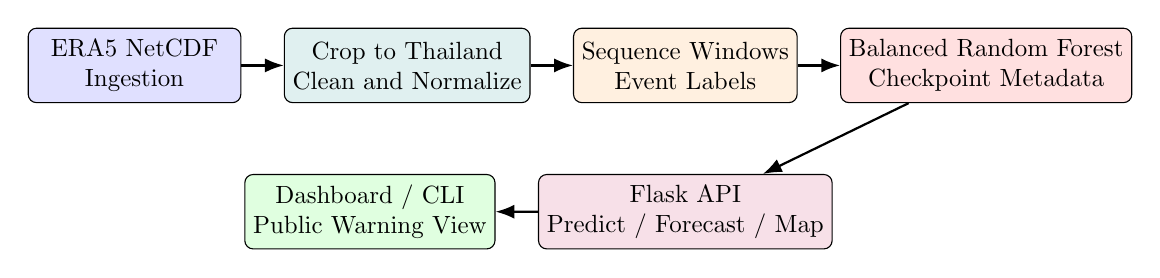
\begin{tikzpicture}[
  scale=0.90,
  transform shape,
  node distance=10mm and 6mm,
  box/.style={draw, rounded corners=3pt, align=center, minimum width=3.0cm, minimum height=1.05cm, fill=#1!12},
  arrow/.style={-{Latex[length=2.4mm]}, thick}
]
\node[box=blue] (data) {ERA5 NetCDF\\Ingestion};
\node[box=teal, right=of data] (prep) {Crop to Thailand\\Clean and Normalize};
\node[box=orange, right=of prep] (features) {Sequence Windows\\Event Labels};
\node[box=red, right=of features] (model) {Balanced Random Forest\\Checkpoint Metadata};

\node[box=purple, below=of features] (api) {Flask API\\Predict / Forecast / Map};
\node[box=green, left=of api] (ui) {Dashboard / CLI\\Public Warning View};

\draw[arrow] (data) -- (prep);
\draw[arrow] (prep) -- (features);
\draw[arrow] (features) -- (model);
\draw[arrow] (model) -- (api);
\draw[arrow] (api) -- (ui);
\end{tikzpicture}
\caption{System architecture of the heatwave prediction and public warning pipeline.}
\label{fig:architecture}
\end{figure}

\section{Results and Evaluation}
\subsection{Checkpoint Used for Reporting}
The quantitative results in this report are taken from the latest available balanced-random-forest checkpoint in the repository, denoted here as \texttt{checkpoint v26}, last modified on March 7, 2026. The stored metadata indicate that the selected event-probability threshold was 0.74 after validation-set tuning. The same checkpoint also records that the training run used a fallback label-selection mode when strict physical thresholds alone did not yield both positive and negative classes. This detail matters because it improves learnability, but it also qualifies how the reported scores should be interpreted.

\subsection{Core Performance Metrics}
Table~\ref{tab:metrics} summarizes the training, validation, and test metrics stored in that checkpoint. The most relevant result for deployment is the test-set F1 score of 0.672, with precision 0.724 and recall 0.626. These values indicate that the system is able to identify a meaningful share of heatwave events while limiting false alarms to a moderate level.

\begin{table}[H]
\centering
\caption{Core event-classification metrics from \texttt{checkpoint v26}.}
\label{tab:metrics}
\begin{tabular}{lcccccc}
\toprule
Split & Accuracy & Precision & Recall & F1 & Brier & PR-AUC \\
\midrule
Train & 0.979 & 0.856 & 0.956 & 0.903 & 0.046 & 0.971 \\
Validation & 0.948 & 0.807 & 0.717 & 0.759 & 0.072 & 0.797 \\
Test & 0.896 & 0.724 & 0.626 & 0.672 & 0.070 & 0.779 \\
\bottomrule
\end{tabular}
\end{table}

\begin{figure}[H]
\centering
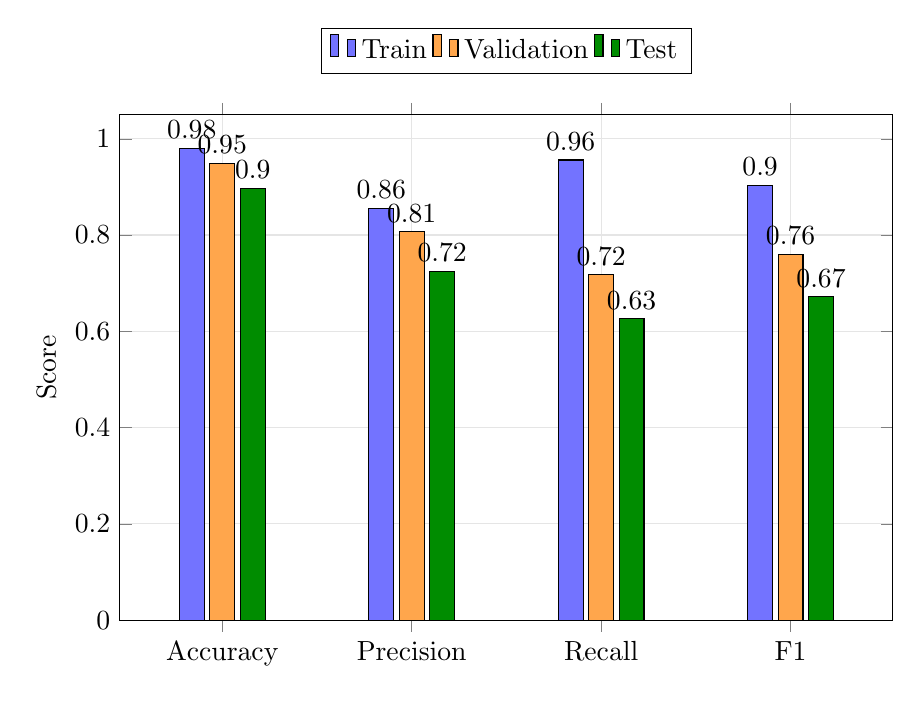
\begin{tikzpicture}
\begin{axis}[
  width=0.94\textwidth,
  height=8cm,
  ybar,
  bar width=9pt,
  ymin=0,
  ymax=1.05,
  ylabel={Score},
  symbolic x coords={Accuracy,Precision,Recall,F1},
  xtick=data,
  legend style={at={(0.5,1.08)}, anchor=south, legend columns=3},
  nodes near coords,
  nodes near coords align={vertical},
  enlarge x limits=0.18,
  grid=major,
  major grid style={draw=gray!20}
]
\addplot[fill=blue!55] coordinates {
  (Accuracy,0.9794)
  (Precision,0.8556)
  (Recall,0.9560)
  (F1,0.9030)
};
\addplot[fill=orange!70] coordinates {
  (Accuracy,0.9482)
  (Precision,0.8068)
  (Recall,0.7172)
  (F1,0.7594)
};
\addplot[fill=green!55!black] coordinates {
  (Accuracy,0.8964)
  (Precision,0.7244)
  (Recall,0.6259)
  (F1,0.6715)
};
\legend{Train,Validation,Test}
\end{axis}
\end{tikzpicture}
\caption{Comparison of classification performance across train, validation, and test splits.}
\label{fig:split-metrics}
\end{figure}

\subsection{Baseline Comparison}
The checkpoint also stores baseline comparisons against persistence and climatology. The learned event classifier is paired with a simple persistence-style temperature baseline for forecasting, but the saved metadata show that persistence and climatology still differ meaningfully in temperature error. Figure~\ref{fig:baseline} summarizes the baseline RMSE and MAE values.

\begin{figure}[H]
\centering
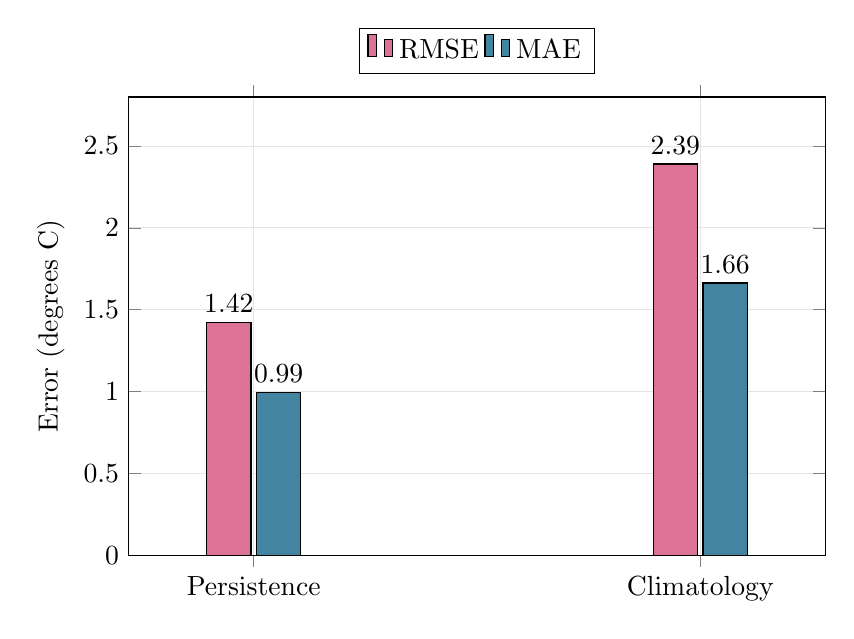
\begin{tikzpicture}
\begin{axis}[
  width=0.86\textwidth,
  height=7.4cm,
  ybar,
  bar width=16pt,
  ymin=0,
  ymax=2.8,
  ylabel={Error (degrees C)},
  symbolic x coords={Persistence,Climatology},
  xtick=data,
  legend style={at={(0.5,1.05)}, anchor=south, legend columns=2},
  nodes near coords,
  enlarge x limits=0.28,
  grid=major,
  major grid style={draw=gray!20}
]
\addplot[fill=purple!55] coordinates {
  (Persistence,1.4226)
  (Climatology,2.3905)
};
\addplot[fill=cyan!60!black] coordinates {
  (Persistence,0.9936)
  (Climatology,1.6628)
};
\legend{RMSE,MAE}
\end{axis}
\end{tikzpicture}
\caption{Temperature-error baselines stored in \texttt{checkpoint v26}. Lower is better.}
\label{fig:baseline}
\end{figure}

\subsection{Regional and Seasonal Variation}
The checkpoint metadata also include grouped evaluation by season and by broad regional bands. These grouped results are useful because heat-risk systems are rarely used uniformly across time and place. In \texttt{checkpoint v26}, the strongest seasonal performance appears during the hot-dry season, where the F1 score reaches 0.731. By contrast, rainy-season performance drops to 0.436, while the cool-dry season contains no positive events under the stored label policy. This pattern suggests that the classifier is learning the dominant warm-season signal well, but that generalization becomes weaker when background meteorology shifts away from the hottest months.

\begin{table}[H]
\centering
\caption{Seasonal event-detection metrics from \texttt{checkpoint v26}.}
\label{tab:seasonal}
\begin{tabular}{lccccc}
\toprule
Season & Accuracy & Precision & Recall & F1 & Positive Count \\
\midrule
Cool-dry & 1.000 & 0.000 & 0.000 & 0.000 & 0 \\
Hot-dry & 0.679 & 0.748 & 0.714 & 0.731 & 112 \\
Rainy & 0.919 & 0.600 & 0.343 & 0.436 & 35 \\
\bottomrule
\end{tabular}
\end{table}

Regional performance shows a similarly uneven pattern. The southern zone reaches the highest regional F1 score at 0.474, followed by the northern zone at 0.426, while the central zone drops to 0.336 despite very high precision. This combination indicates that the classifier is conservative in central Thailand: when it predicts an event it is usually correct, but it misses many true events. Figure~\ref{fig:regional-f1} summarizes this regional imbalance.

\begin{figure}[H]
\centering
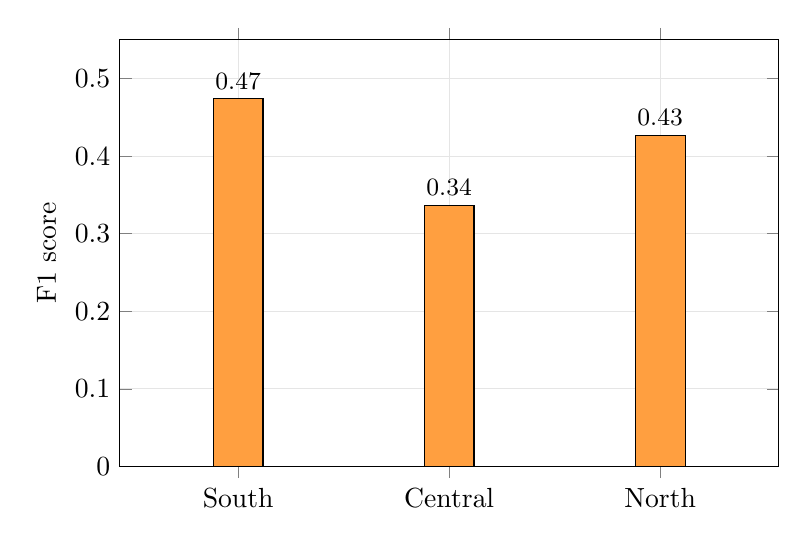
\begin{tikzpicture}
\begin{axis}[
  width=0.82\textwidth,
  height=7.0cm,
  ybar,
  bar width=18pt,
  ymin=0,
  ymax=0.55,
  ylabel={F1 score},
  symbolic x coords={South,Central,North},
  xtick=data,
  nodes near coords,
  enlarge x limits=0.28,
  grid=major,
  major grid style={draw=gray!20},
  every node near coord/.append style={font=\small}
]
\addplot[fill=orange!75] coordinates {
  (South,0.4738)
  (Central,0.3364)
  (North,0.4264)
};
\end{axis}
\end{tikzpicture}
\caption{Regional F1 scores from \texttt{checkpoint v26}.}
\label{fig:regional-f1}
\end{figure}

\subsection{Cost Analysis and Scalability}
The current backend is relatively cost-efficient because the operational training path is CPU-friendly. This reduces hardware requirements compared with training a full deep spatiotemporal model for every update cycle. The data loader also lowers memory cost by cropping to Thailand before merging files and by preferring lazy \texttt{xarray} loading when available. These design choices make the system suitable for prototype deployment in education, municipal warning support, or lightweight research settings.

At the same time, scalability remains a practical limitation. The Flask service stores model state, cached sequences, and normalization statistics in module-level memory. This is acceptable for a demonstration environment but less ideal for large concurrent workloads. The map endpoint also emits one polygon per grid cell, which could become bandwidth-heavy at higher spatial resolution. Future production scaling should therefore emphasize shared model services, containerized workers, and more compact spatial data delivery.

\subsection{Interpretation}
The results suggest that the system is most credible when positioned as a heatwave-risk support tool rather than as a perfect deterministic forecast. The test metrics show useful signal, especially in precision and PR-AUC, but they also show that some events will still be missed. This reinforces the value of presenting the output as risk levels, probabilities, and public guidance instead of as an absolute yes-or-no guarantee.

\section{Discussion and Limitations}
The present implementation already demonstrates a coherent environmental-AI workflow, but it also reveals several limitations that should be stated explicitly in a serious paper. First, the deployed training backend is a flattened-feature classifier, so it does not yet preserve the full spatial structure of the weather fields. Second, the reported checkpoint used a fallback label-generation mode, which is operationally practical but indicates that the physical event definition and the observed data distribution do not always align cleanly. Third, the available evaluation is model-centric rather than impact-centric. The repository measures predictive performance, but it does not yet validate whether the warnings improve user decisions, reduce exposure, or align with observed health outcomes.

There are also system-design limitations. The current Flask service keeps model state and caches in process memory, which is acceptable for a prototype but not ideal for large-scale deployment. In addition, the map endpoint emits one polygon per grid cell, which can become heavy as the grid resolution increases. The grouped results in Table~\ref{tab:seasonal} and Figure~\ref{fig:regional-f1} further suggest that the model behaves differently across seasons and regions, so deployment should avoid assuming uniform reliability across Thailand. From a scientific standpoint, future work should evaluate the system across more years, test alternative event definitions, examine calibration and reliability more closely, and compare results against stronger imbalance-aware baselines under the same data split and label policy.

\section{Environmental Impact}
The project has a potentially positive environmental and social impact because earlier awareness of dangerous heat conditions can help communities reduce harmful exposure, improve preparedness, and support adaptation planning. Heat-risk maps and warning levels can also make climate information more actionable for schools, households, and local decision makers. At the same time, AI-enabled environmental systems have their own resource costs, including compute, storage, and data-transfer overhead. The current design partially mitigates those costs by using a relatively efficient CPU-oriented backend, spatial cropping, and lazy loading for large climate files. This makes the system more realistic for low-cost deployment contexts while still leaving room for future optimization.

\section{Conclusion}
Heatwave Heat Map Life demonstrates how environmental data, machine learning, and public communication can be combined into a practical warning pipeline for Thailand. The implemented system ingests ERA5 data, derives spatiotemporal features, trains an imbalance-aware classifier, and exposes results through an API that supports dashboards and map-based warnings. The latest checkpoint indicates that the model can detect heatwave events with meaningful skill while maintaining manageable error levels.

The next step is not merely to chase a higher score, but to improve scientific validity and operational usefulness at the same time. That means refining label definitions, expanding evaluation, and introducing user-centered validation. With those improvements, the project could evolve from a promising prototype into a more credible heat-risk intelligence system for Thailand.

\section*{Note on Metric Provenance}
All numeric values in the plots and tables above were extracted from the metadata stored in \texttt{checkpoint v26}. They reflect the repository state available on March 7, 2026.

\begin{thebibliography}{99}

\bibitem{hersbach2020}
Hersbach, H., Bell, B., Berrisford, P., et al. (2020).
\newblock The ERA5 global reanalysis.
\newblock \emph{Quarterly Journal of the Royal Meteorological Society}, 146(730), 1999--2049.
\newblock doi: \href{https://doi.org/10.1002/qj.3803}{10.1002/qj.3803}

\bibitem{breiman2001}
Breiman, L. (2001).
\newblock Random forests.
\newblock \emph{Machine Learning}, 45(1), 5--32.
\newblock doi: \href{https://doi.org/10.1023/A:1010933404324}{10.1023/A:1010933404324}

\bibitem{chen2004}
Chen, C., Liaw, A., \& Breiman, L. (2004).
\newblock Using Random Forest to Learn Imbalanced Data.
\newblock Technical Report 666, Department of Statistics, University of California, Berkeley.
\newblock Available at: \url{https://digicoll.lib.berkeley.edu/record/85556}

\bibitem{chandra2025}
Chandra N, S. V. S., \& Lee, J. K. W. (2025).
\newblock A systematic review of heat health warning systems: enhancing the framework towards effective health outcomes.
\newblock \emph{Current Environmental Health Reports}, 12, Article 31.
\newblock doi: \href{https://doi.org/10.1007/s40572-025-00496-5}{10.1007/s40572-025-00496-5}

\bibitem{toloo2013}
Toloo, G. S., FitzGerald, G., Aitken, P., Verrall, K., \& Tong, S. (2013).
\newblock Are heat warning systems effective?
\newblock \emph{Environmental Health}, 12, Article 27.
\newblock doi: \href{https://doi.org/10.1186/1476-069X-12-27}{10.1186/1476-069X-12-27}

\bibitem{whoheat}
World Health Organization. (2024).
\newblock Heat and health.
\newblock Available at: \url{https://www.who.int/mega-menu/health-topics/popular/excessive-heat}

\end{thebibliography}

\end{document}
